\chapter{IBM BigFix}

\section{BigFix}
I prodotti della suite IBM BigFix consentono di monitorare e gestire in tempo reale un elevato numero di dispositivi fisici e virtuali connessi (fino a 250.000). Questi possono essere sia fisici che virtuali, come ad esempio server, desktop, notebook, dispositivi mobili, tablet, POS, ATM, chioschi self-service. Gli utenti principali di questi prodotti sono gli amministratori di sistema. Tramite le applicazioni BigFix possono avere il pieno controllo sugli endpoint, come distribuire software, applicare delle patch, effettuare il deploy di sistemi operativi, proteggere da attacchi di rete e molto altro.
\subsection{Architettura}
Un'architettura di BigFix è, per sua natura, molto articolata, poichè la necessità e quella di gestire un numero elevato ed eterogeneo di dispositivi. Essa si basa sul consolidato pattern stilistico Client/Server, ma con una struttura leggermente variata, prevedendo l'inserimento di un ulteriore layer frapposto tra client e server, i relay, i quali sono fondamentali per bilanciare il carico.
\paragraph{}
Ma partiamo subito con un esempio per avere un ponto di riferimento.
\begin{figure}[h!]
	\centering
	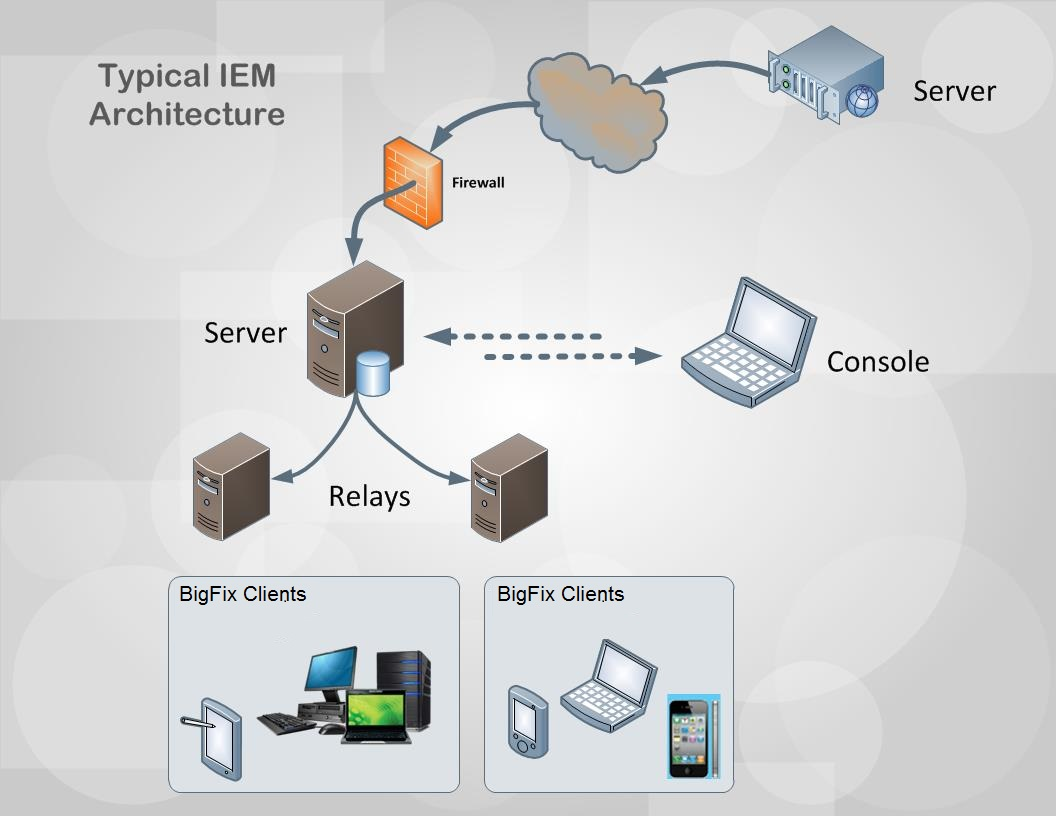
\includegraphics[width=\textwidth,keepaspectratio=true]{capitoli/imgs/IEMArchitecture.png}
	\caption{Un'architettura BigFix di esempio}
\end{figure}
Come possiamo notare, l'elemento fondamentale è il server, il quale ha lo scopo di raccogliere dei particolari messaggi, le Fixlet. Questi messaggi posso essere visualizzati dall'operatore che lavora sulla console e inoltrati quindi, a questo punto ai relay. E' competenza dei relay poi interagire con i singoli client e assicurarsi l'esecuzione delle Fixlet. Le Fixlet, infatti, altro non sono che delle azioni che devono essere necessariamente compiute dai client.
Andiamo ad analizzare le singole componenti dell'archiettura.
\paragraph{Servers}
Il server coordina tutto il flusso di informazioni e si preoccupa di salvare le informazioni sul database. Al tempo stesso però, lascia agli Agent il compito di effettuare analisi ed eseguire azioni specifiche. Ciò consente di liberare il Server da un pesantissima computazione. Per questo motivo il Serve stesso può gestire al altissimo numero di client.
\paragraph{Relays}
I Relay si comportano come una cache tra i Client e il Server e sono di numero variabile in base al numero di Client. Aiutano il Server a gestire i dispositivi anche se funzionalmente non sono altro che Client che sono stati promossi a Relay, aggiungendo a loro dei servizi. A questo punto i Client non si interfacceranno mai con il Server, alleggerendone così notevolmente il workload. Possono, ad esempio, più Client richiedere un download al Relay, il quale effettuerà un'unica richiesta al Server
\paragraph{Agents}
Un Agent è installato su ogni Client facente parte dell'architettura di BigFix. essi hanno il compito di raccogliere le Fixlet, tramite le quali sono in grado, ad esempio, di individuare e correggere le exposure di sicurezza, configurazioni scorrette e altre vulnerabilità. Fa dei continui check per confrontare lo stato del dispositivo con le policy stabilite. Appena scopre che il dispositivo è fuori dalla compliance, viene informato il Server ed agisce subito per porre rimedio e, al termine, informa nuovamente sull'esito dell'operazione.
\paragraph{Web Reports}
I Web Reports sono il componente che consentono ad utenti autorizzati di monitorare tutti i dispositivi di BigFix. SI piò in questo modo tenere traccia di vulnerabilità, azioni richieste e molto altro.
\paragraph{Consoles}
La Console permette agli amministratori di interagire con tutti i Client dell'ambiente BigFix. Gli utenti possono così distribuire velocemente patch e configurazioni.
\paragraph{}
BigFix, da un punto di vista logico, si suddivide in due grandi macro-componenti, la Platform e le Applications. La prima svolge la funzione di layer sulla quale vengono sviluppate tutte le funzionalità dello strato di applications. Questa suddivisione consente una chiara suddivisione delle competenze da parte di progettisti, sviluppatori, tester e assistenti dei clienti. Il team della platform si concentra quindi nel fornire una solida infrastruttura al team delle applications, il quale svilupperà i singoli strumenti al servizio dell'utente.
\subsection{BigFix Platform}
La Platform è una tecnologia multi-layer scritta in linguaggio C++ che agisce come colonna portante di tutta l'infrastruttura di BigFix. La Platform svolge infatti funzioni fondamentali, spesso utilizzate anche da altre applicazioni dei layer superiori. La Platform divide le responsabilità.
\paragraph{Lifecycle Management}
Include il controllo remoto, la distribuzione dei softawre e il deploy di sistemi operativi.
\paragraph{Patch Management}
Consente l'applicazione e la gestione delle patch.
\paragraph{Core Protection}
E' il cuore di tutta la routine di Security. Troviamo quì delle funzionalità anti-malware, firewall e protezione da qualsiasi variante di virus.
\paragraph{Inventory }
Raccoglie informazioni peculiari a riguardo dei software installati su ogni dispositivo. E' in grado di effettuare analisi sugli utilizzi fornendo una base per la decisione sulle licenze da acquistare.
\paragraph{Server Automation}
Fornisce un Hypervisor per le Virtual Machines. Esso controlla infatti eventuali malfunzionamenti degli ambienti virtuali.
\subsection{BigFix Applications}
Tutti i prodotti applicativi che fanno parte di questo componente consentono di gestire in maniera semplice tutte le operazioni inerenti alla security. A differenza della Platform sono implementate in linguaggio Java ed hanno funzionalità atomiche tra di loro. Sono l'interfaccia principale con il quale interagisce l'amministratore aziendale.
\subsection{Fixlets}
Le Fixlet sono il metodo attraverso il quale si svolgono tutte le operazioni come distribuzione di software, installazioni di patch e configurazioni. Esse sono dei messaggi inoltrati ai client di BigFix e utilizzano un linguaggio di query specifico, il Relevance.
\subsubsection{Il linguaggio Relevance}
Con una Fixlet si può anche ispezionare un desiderato aspetto di un client. Il linguaggio di Relevance consente di interrogare il client identificandone caratteristiche dell'hardware o del software tramite gli Inspectors. Una necessità può essere infatti quella di applicare una Fixlet solamente a dei client con determinate caratteristiche hardware/software oppure che si trovano in stati ben definiti. Si può in questo modo, facilmente identificare il corretto sottoinsieme di client ai quali è destinata una nuova Fixlet ed applicarla solo ad essi.

\section{IBM}
Il lavoro di tesi si è svolto nell'ambito di un progetto formativo stipulato tra l'Università dell'Aquila e IBM Italia Spa. Questo progetto ha previsto un tirocinio svolto nella seda di Roma con obiettivo: "Esplorazione e prototipazione di metodi per portare prodotti BigFix su cloud", per l'appunto la realizzazione del prototipo di BigFix Saas. 


